% Created 2021-12-09 Thu 18:31
% Intended LaTeX compiler: pdflatex
\documentclass[presentation]{beamer}
\usepackage[utf8]{inputenc}
\usepackage[T1]{fontenc}
\usepackage{graphicx}
\usepackage{longtable}
\usepackage{wrapfig}
\usepackage{rotating}
\usepackage[normalem]{ulem}
\usepackage{amsmath}
\usepackage{amssymb}
\usepackage{capt-of}
\usepackage{hyperref}
\usetheme{metropolis}
\usepackage[UTF8]{ctex}
\usepackage{caption}
\usepackage{csquotes}
\usepackage{subcaption}
\usepackage[font=itshape]{quoting}
\usetheme{default}
\author{田壮志,朱开,张青,张劲波,郭慧子,张登富,陈淇奥}
\date{\today}
\title{老龄化}
\hypersetup{
 pdfauthor={田壮志,朱开,张青,张劲波,郭慧子,张登富,陈淇奥},
 pdftitle={老龄化},
 pdfkeywords={},
 pdfsubject={},
 pdfcreator={Emacs 27.2 (Org mode 9.6)}, 
 pdflang={English}}
\begin{document}

\maketitle

\section{老龄化的一些事例}
\label{sec:orgb6e9242}
\begin{frame}[label={sec:orgd52673a}]{市东敬老院}
\begin{columns}[onlytextwidth,T]
  \column{\dimexpr\linewidth-50mm-5mm}
市东敬老院是邯郸校区北区东侧的一家养老院,与宿舍区仅有一墙之隔。
  \column{50mm}
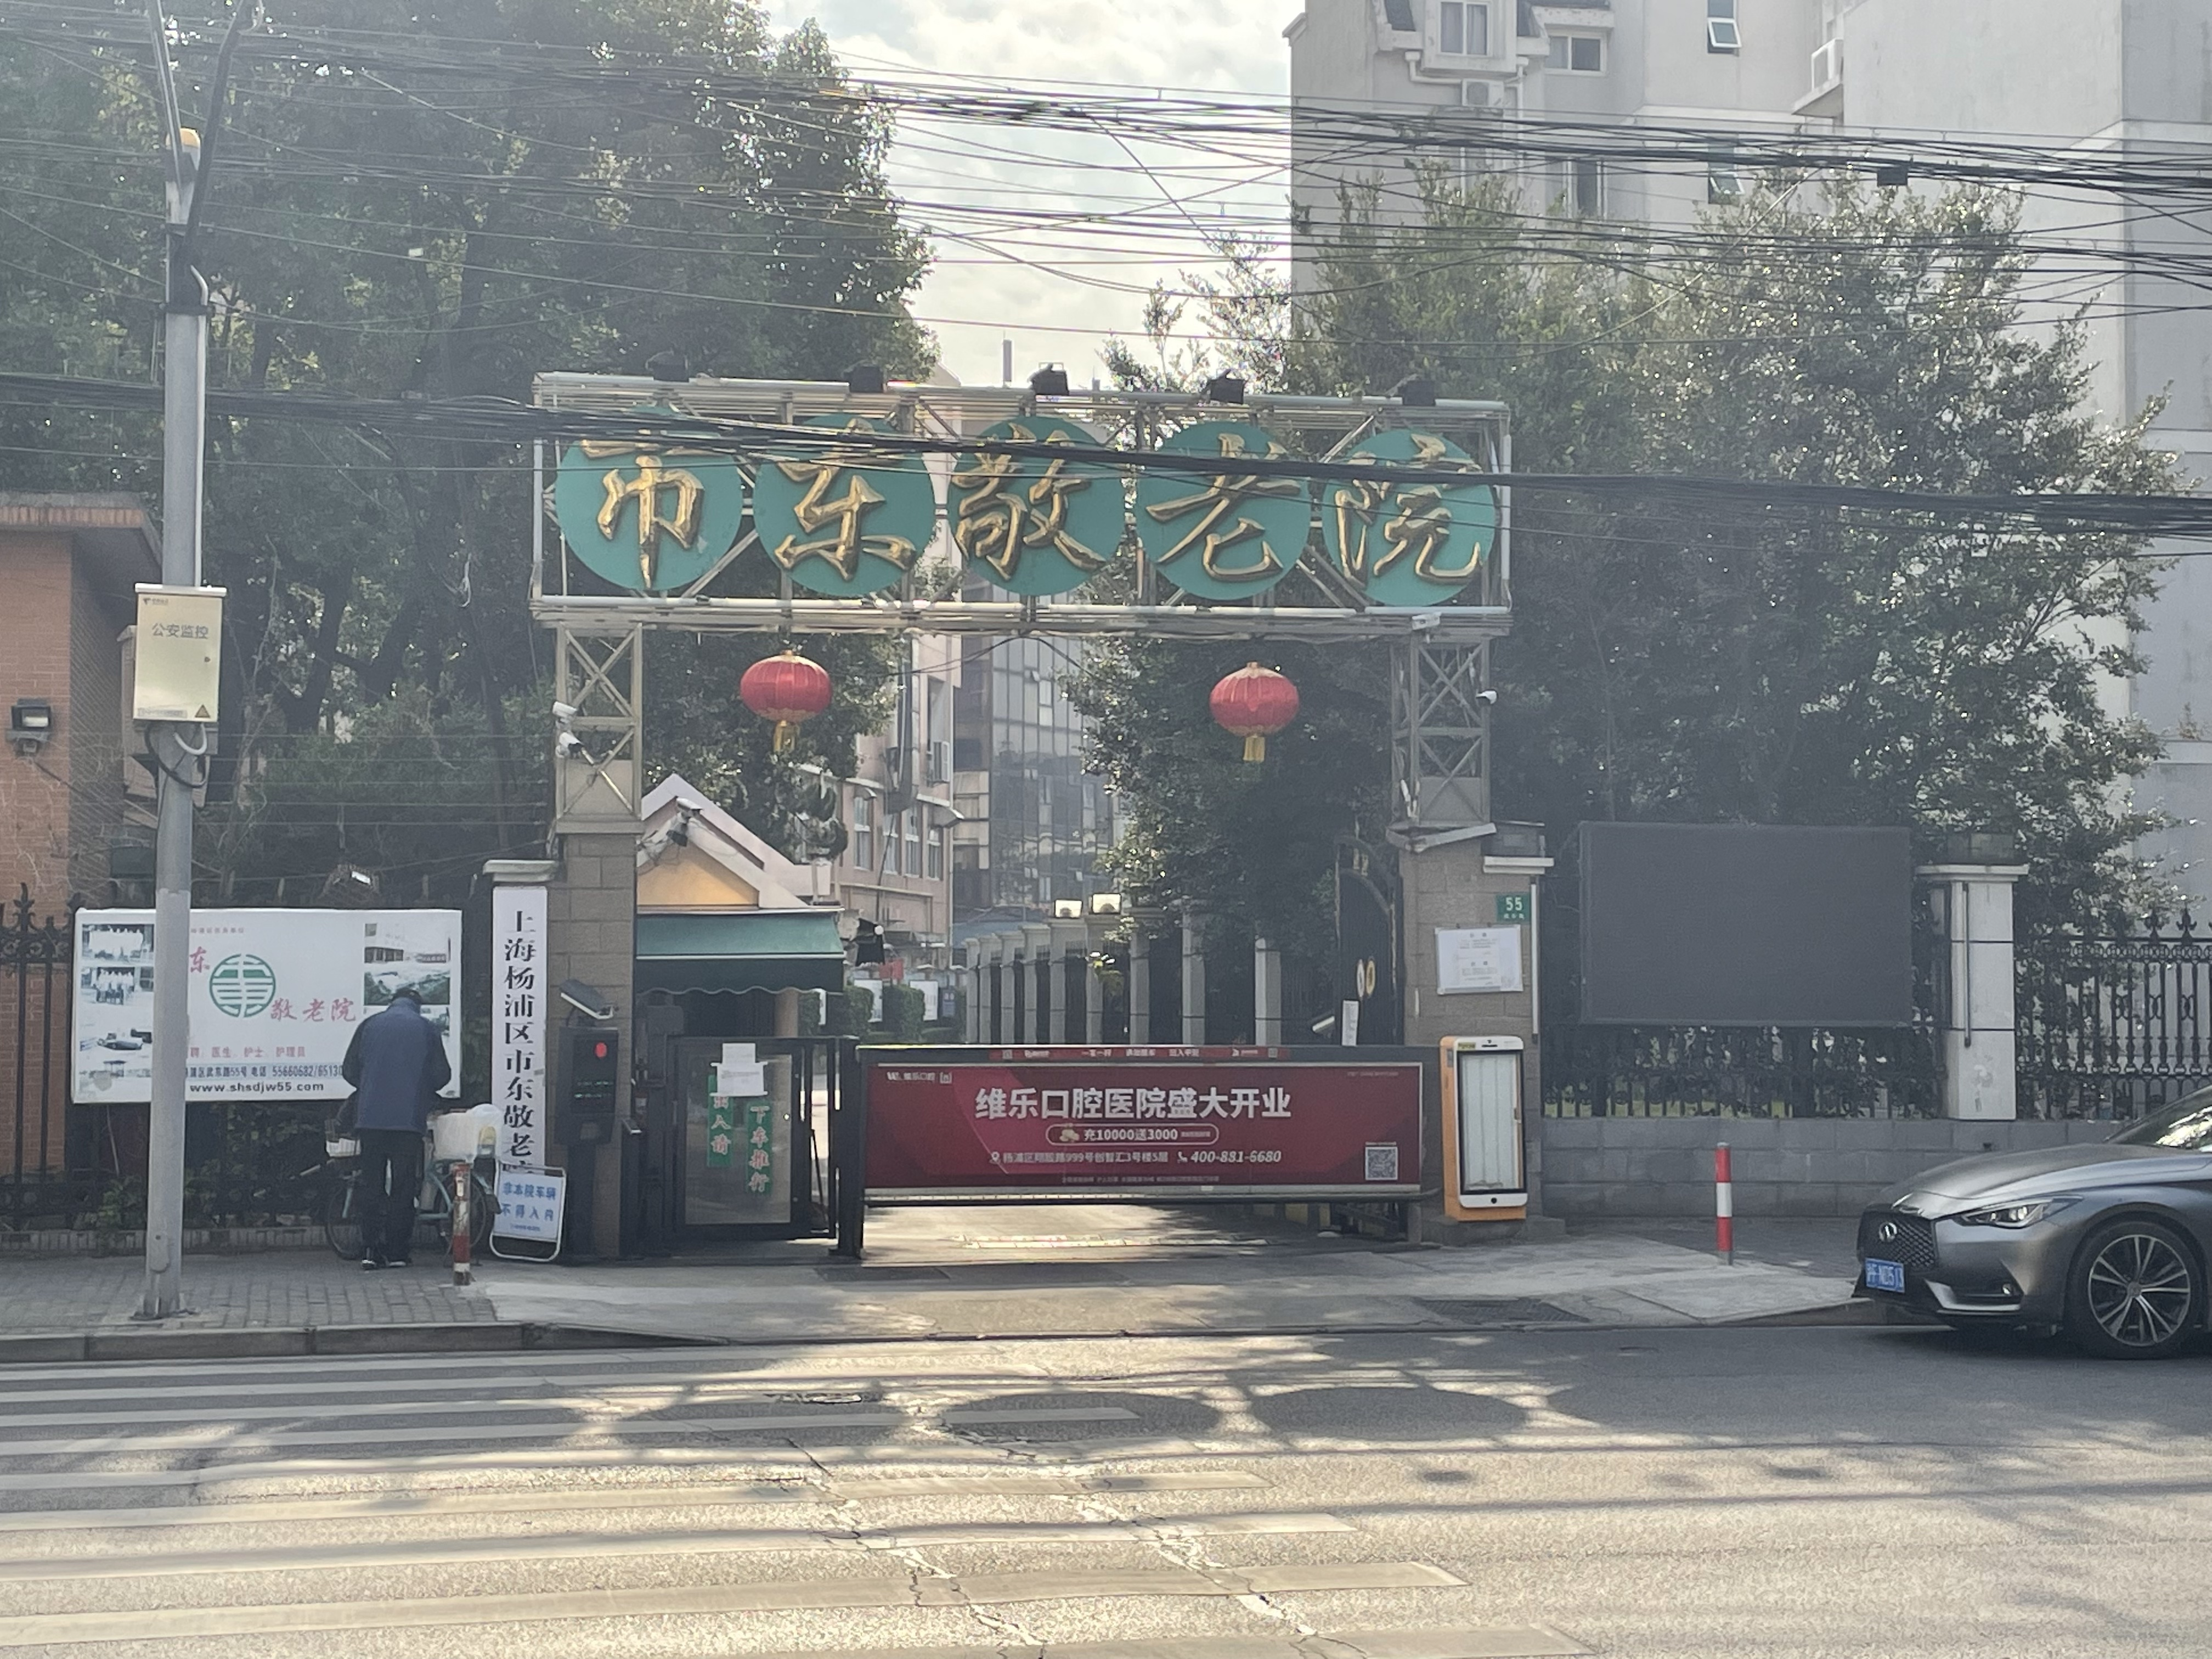
\includegraphics[width=50mm]{3}
\end{columns}
\end{frame}
\begin{frame}[label={sec:orgdf90e72}]{市东敬老院}
\begin{figure}[ht]
    \begin{minipage}[b]{0.45\linewidth}
        \centering
        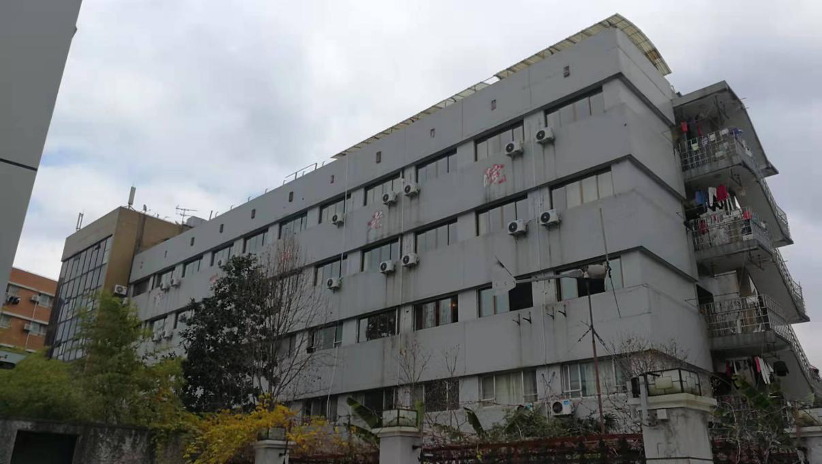
\includegraphics[width=\textwidth]{2}
        \caption*{市东敬老院}
        \label{fig:a}
    \end{minipage}
    \hspace{0.5cm}
    \begin{minipage}[b]{0.45\linewidth}
        \centering
        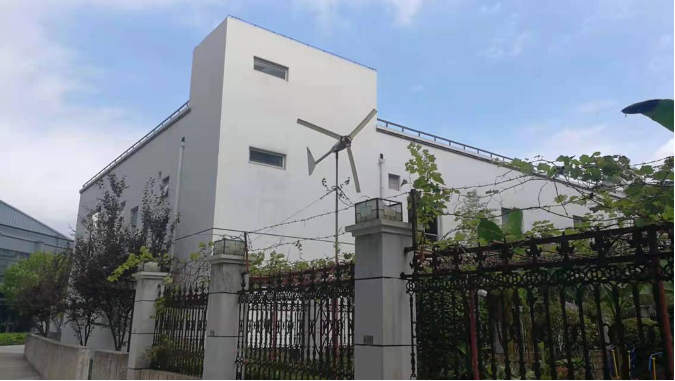
\includegraphics[width=\textwidth]{1}
        \caption*{青书馆}
        \label{fig:b}
    \end{minipage}
\end{figure}
\end{frame}

\begin{frame}[label={sec:org18d26bf}]{​}
上面是上海养老院的一个例子,它给我们提供了一个对当今社会年龄结构的最直观印象。既然上海是这
样,那么在其它地方,尤其在农村,情况又怎么样呢?
\end{frame}

\begin{frame}[label={sec:org1d9d777}]{A村}
18年夏天,7月底到8月初,组内有同学曾在湖南省湘西州古丈县的A村里做过为期两周的定点田野调查。

A村地处国家级贫困县,包括两个自然村,当时正是全面脱贫攻坚完成前的最后一年。

\begin{figure}
\centering
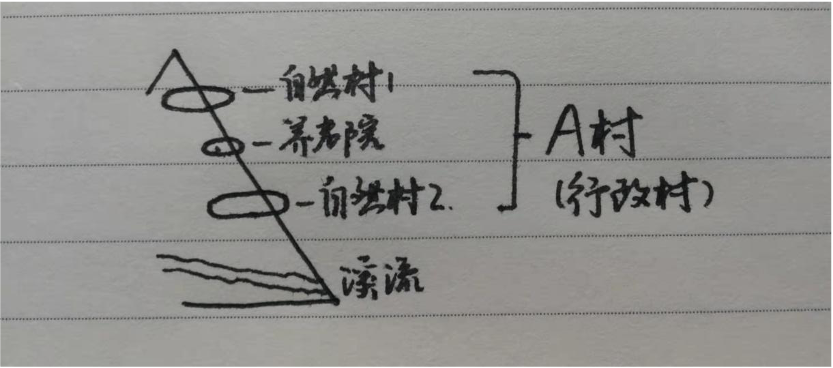
\includegraphics[width=.7\textwidth]{4}
\caption*{A村地形图}
\end{figure}
\end{frame}

\begin{frame}[label={sec:orgf2d6dd6}]{A村}
根据村支两委提供的数据,整个行政村只有196户居民,合计716人。但在调查期间,村里能碰上人的(包括养
老院)大概不足20户;并且多以老人为主。小孩就碰到一个,在县城上小学,当时正放暑假在家。\pause

整个村子基本快空了。
\end{frame}
\begin{frame}[label={sec:org4e1b925}]{A村}
\begin{figure}
    \centering
    \begin{subfigure}[b]{0.48\textwidth}
        \centering
        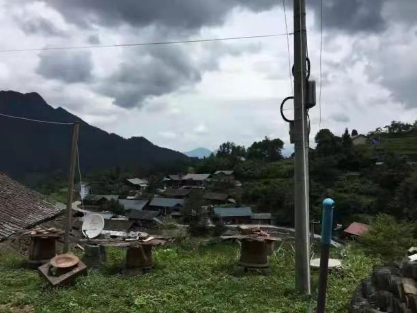
\includegraphics[width=\textwidth]{11}
    \end{subfigure}
    \hfill
    \begin{subfigure}[b]{0.48\textwidth}
        \centering
        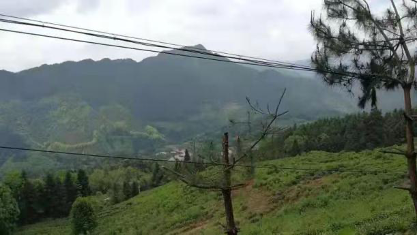
\includegraphics[width=\textwidth]{12}
    \end{subfigure}
    \vskip\baselineskip
    \begin{subfigure}[b]{0.48\textwidth}
        \centering
        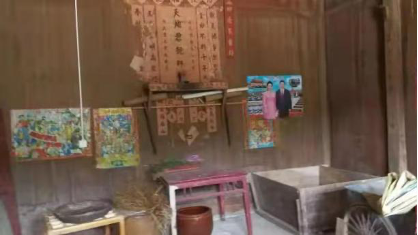
\includegraphics[width=\textwidth]{13}
    \end{subfigure}
    \hfill
    \begin{subfigure}[b]{0.48\textwidth}
        \centering
        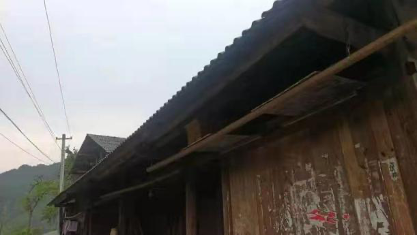
\includegraphics[width=\textwidth]{14}
    \end{subfigure}
\end{figure}
\end{frame}
\begin{frame}[label={sec:org7ec04a6}]{两个事例给出的一些信息}
农村里基本只剩老人(就中西部山区来看);城市里也面临老龄化问题,这是一个当下中国不得不面对的事实。
\end{frame}
\section{数据}
\label{sec:org9131e73}
\begin{frame}[label={sec:org8d3178a}]{​}
\begin{figure}[htbp]
\centering
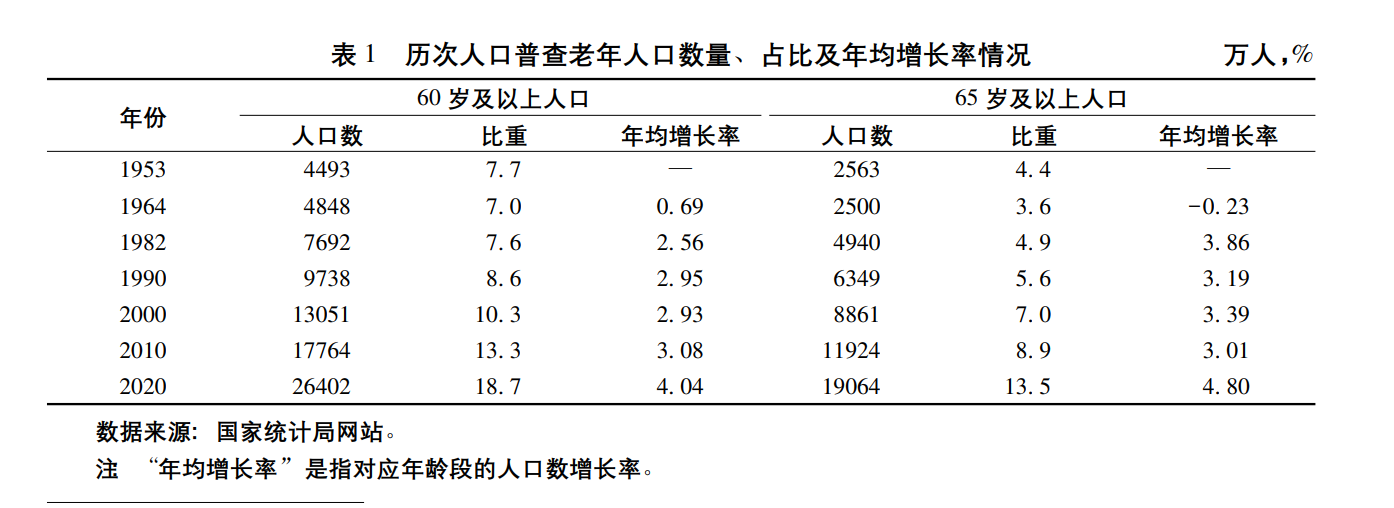
\includegraphics[width=.99\textwidth]{./5.png}
\label{}
\end{figure}
\end{frame}
\begin{frame}[label={sec:orgf2cd1e6}]{​}
\begin{figure}[htbp]
\centering
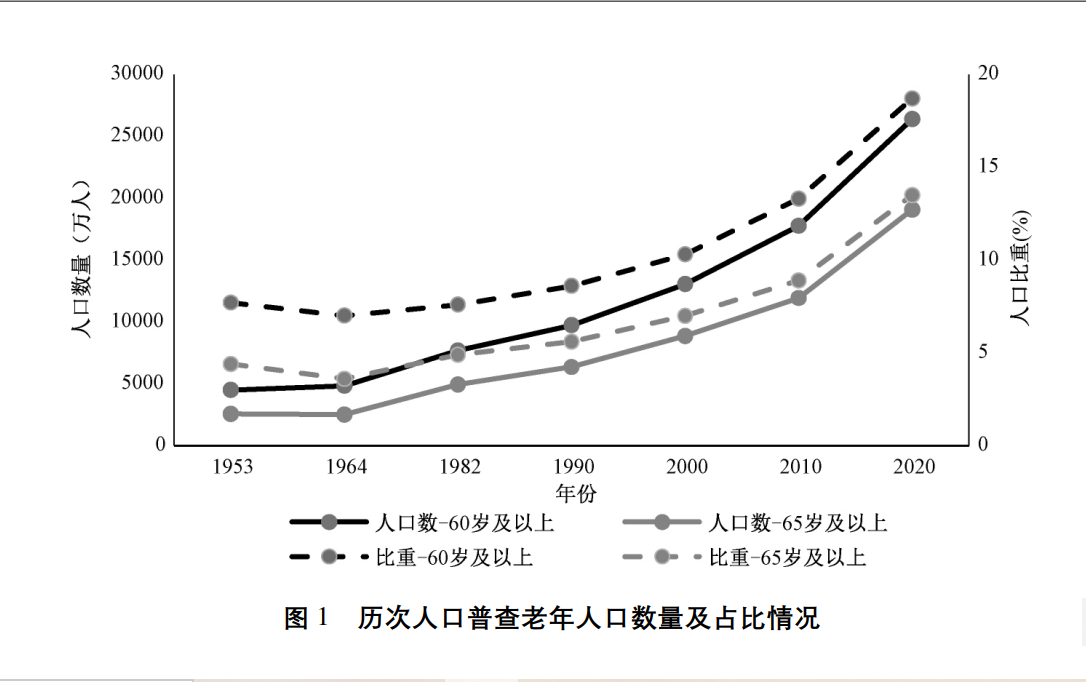
\includegraphics[width=.99\textwidth]{./6.png}
\label{}
\end{figure}
\end{frame}
\begin{frame}[label={sec:org5cd4f8c}]{​}
\begin{figure}[htbp]
\centering
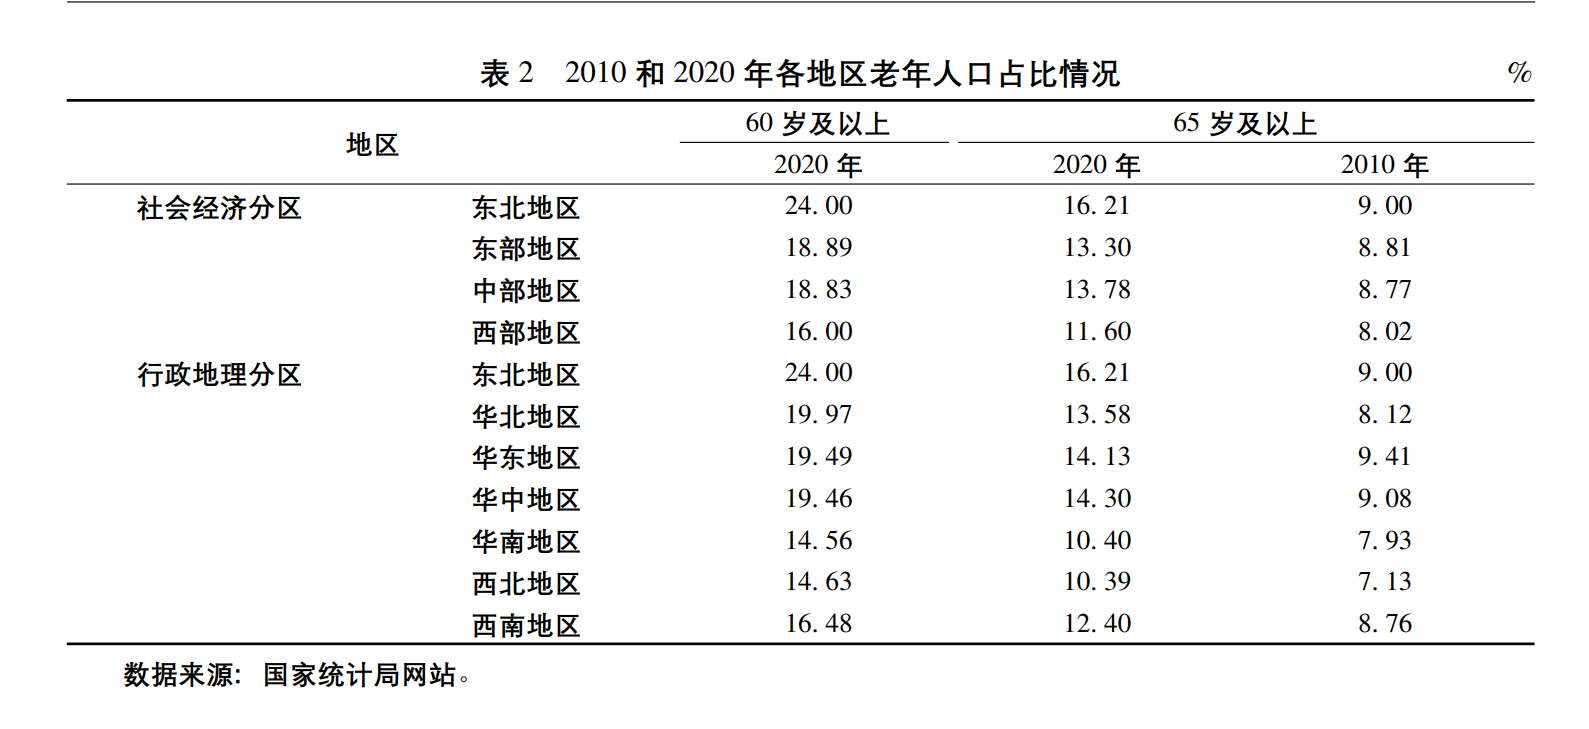
\includegraphics[width=.99\textwidth]{./7.png}
\label{}
\end{figure}
\end{frame}
\begin{frame}[label={sec:org18d29be}]{​}
\begin{figure}[htbp]
\centering
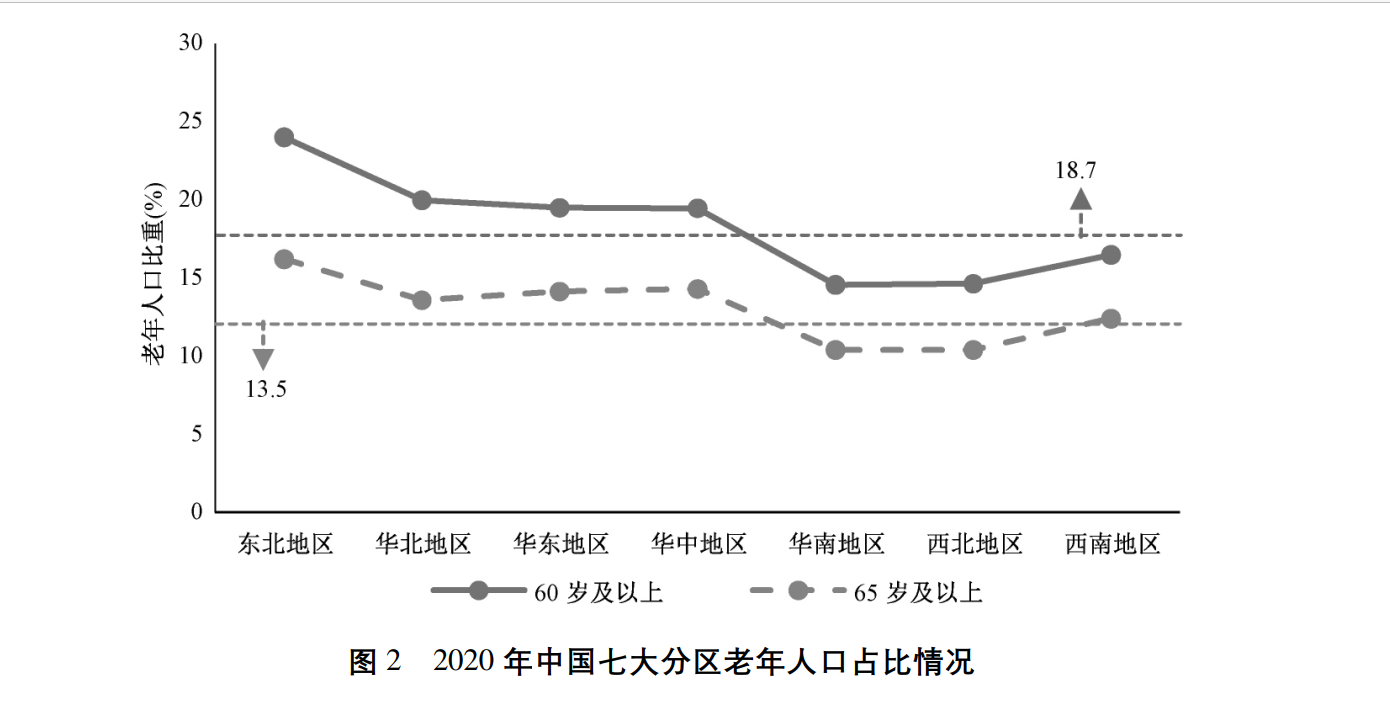
\includegraphics[width=.99\textwidth]{./8.png}
\label{}
\end{figure}
\end{frame}
\begin{frame}[label={sec:orgc0e4e1e}]{​}
\begin{figure}[htbp]
\centering
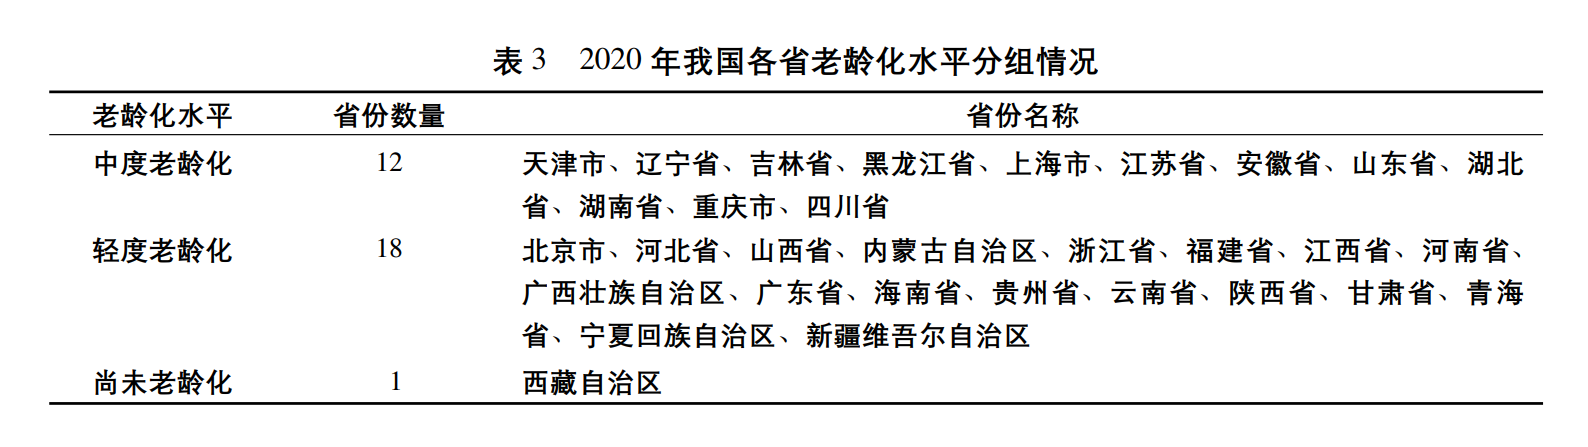
\includegraphics[width=.99\textwidth]{./9.png}
\label{}
\end{figure}
\end{frame}

\section{现状、思考及拓展}
\label{sec:org81cc497}
\begin{frame}[label={sec:org46dd89e}]{根本:生生生}
\begin{quoting}
{\footnotesize 47.实施积极应对人口老龄化国家战略。制定人口长期发展战略,优化生育政策,增强生育政策包容性,提高优生优育服务水平,发展普惠托育服务体系,降低生育、养育、教育成本,促进人口长期均衡发展,提高人口素质。积极开发老龄人力资源,发展银发经济。推动养老事业和养老产业协同发展,健全基本养老服务体系,发展普惠型养老服务和互助性养老,支持家庭承担养老功能,培育养老新业态,构建居家社区机构相协调、医养康养相结合的养老服务体系,健全养老服务综合监管制度。}
\end{quoting}

应对老龄化问题,归根结底是要能 \alert{多生} 。
\end{frame}
\begin{frame}[label={sec:orgca3ed6d}]{根本:生生生}
那么,能否通过社会化养老促进多生呢?大家不妨问自己两个问题:
\begin{enumerate}
\item 自己家里是怎么养老的?
\item 什么是社会化养老?——拿后一辈的钱养前一辈\pause
\end{enumerate}


关键在第二个问题:一切的一切都在于,要有人养老,也就是生育率要能上去。
\end{frame}
\begin{frame}[label={sec:orgdce945b}]{根本:生生生}
\begin{enumerate}
\item 不管我们对家庭结构怎么看,社会化养老都解决不了问题。
\item 应对老龄化的根本在于生育率的提高。\pause
\end{enumerate}


但是我们有一个矛盾
\begin{align*}
\text{老人要养老}&\longrightarrow\text{需要一定的生育率}\\
\text{独生子女一代压力大}&\longrightarrow\text{没有生育意愿}
\end{align*}
\end{frame}
\begin{frame}[label={sec:orgdab71b3}]{内核:家庭}
生育率提高的核心在于家庭,这是一个牵涉到经济社会政治思想文化各方面因素的复杂问题,需要严肃的专门
讨论。下面我们要摆出的,是面对“家庭”这样一个复杂问题,国家现在到底怎么看的。\pause

《民法典草案》第1045条:直系近亲属(2019年;现已删去)
\begin{figure}[htbp]
\centering

\includegraphics[width=.7\textwidth]{./10.png}
\label{}
\end{figure}
\end{frame}
\begin{frame}[label={sec:org7999fb4}]{哲学中家的概念}
家概念在中国哲学中华文明几千年的漫长历史中始终占有中心位置。以儒家为中心的东方家哲学是世界上
最古老、最发达的家哲学之一。围绕“阴—阳”、“孝、悌”这些观念建立起来的家哲学是中国哲学的精华部分。\pause

家哲学对于东亚就像水对于舟的关系一样既有好的(载舟)一面也可以有不好的(覆舟)一面。由东亚近两个
世纪与西方交往的经历看我们主要看到的是东方家文化覆舟的一面———例如对中国人个性意识和公共精神的压
制。\pause

只有站在不含这种水的地中海岸边观察时我们才会发现家庭文化这种水除了覆舟之外还有载舟的积极功能。
\end{frame}
\begin{frame}[label={sec:orge5231f5}]{哲学中家的概念}
我们站在现时代对于“家”问题进行深入探讨,希望有能力来论述现代社会中的家问题。“家”是一个母题,是一
个原型,这里既有如何面对现代世界再造家庭之挑战的问题,也有如何在现代社会建构“家外之家”的问题,比
如福利社会。黑格尔针对社会所说的“第二家庭”或“普遍家庭”等概念就已经有福利社会的影子。\pause
\end{frame}


\begin{frame}[label={sec:orgdd8fcd6}]{提高生育率的可能对茦}
\begin{enumerate}
\item 给予产假、育儿假、男方陪产假等假期保障。

意大利产妇享有22周的产假和26周的育儿假;德国和日本产妇享有14周的产假和44周的育儿假\(\dots\)
\item 给予现金补助、税收返还等经济补贴。

法国为一孩生育提供一次性补助941欧元和3岁前每月补助85欧元,此后随着孩子增加而增多\(\dots\)
\end{enumerate}
\end{frame}

\begin{frame}[label={sec:org4cadc1f}]{提高生育率的可能对茦}
\begin{enumerate}
\setcounter{enumi}{2}
\item 完善托幼服务体系

德国推行“多代屋”计划,鼓励不同家庭、不同年龄的人住在一起\(\dots\)
\item 为女性提供更多就业支持。

法国企业为员工提供灵活的工作时间和最低工作时间,推广在家工作\(\dots\)
\item 推动家庭和工作的平衡。

法国企业为员工提供灵活的工作时间和最低工作时间,推广在家工作\(\dots\)
\end{enumerate}
\end{frame}

\begin{frame}[label={sec:org397793f}]{​}
  \centering \Large
\emph{谢谢}
\end{frame}
\end{document}
